\documentclass[english]{eqconf}
\usepackage[T1]{fontenc}
\usepackage[utf8]{inputenc}
%\usepackage{showframe}
\usepackage{babel}
\usepackage{graphicx}
\usepackage[labelfont=bf,textfont=md]{caption} 
\DeclareCaptionLabelSeparator{period-newline}{.}
 \captionsetup[figure]{labelfont={bf},name={Figure},labelsep=period}
\captionsetup[table]{labelfont={bf},name={Table},labelsep=period}


\usepackage{blindtext} 
 
\title{BİLDİRİ BAŞLIĞI\vspace{2pt}}
\author{\textbf{%
		Mücahit Bekin\textsuperscript{1} ve
		Barış Erkuş\textsuperscript{2}\vspace{1pt}%
}}

\date{\small%
\textsuperscript{\textbf{1}}
\textit{Prof. Dr., İnşaat Müh. Bölümü, Abece Üniversitesi, Güzelkent}\\
\textsuperscript{\textbf{2}}
\textit{Araş. Gör., Jeofizik Müh. Bölümü, Abece Teknik Üniversitesi, 
Büyükkent}\\
\textit{Email: gönderenyazar@kurum}%
}

 
\begin{document}
 
\maketitle

 \thispagestyle{firststyle}
 
\begin{ozet}   %%% A Turkish Abstract has to be provided if the paper is in Turkish
	
\blindtext

\textbf{ANAHTAR KELİMELER:} Anahtar Kelime

\end{ozet}

\begin{abstract} %%% All papers (both Turkish and English) have to provide English abstract
	
	\blindtext
	
\textbf{KEYWORDS:} Anahtar Kelime
	
\end{abstract}

\vspace{1em}
 
\section{INTRODUCTION}
 
The Monty Hall problem...
$x=\frac{a}{b}$
 
\subsection{Theory}

\blindtext

\section{INTRODUCTION}

\blindtext

\subsubsection*{Theory}

\blindtext

\blindtext

\blindtext

\blindtext

\blindtext


\begin{figure}
	\begin{center}
		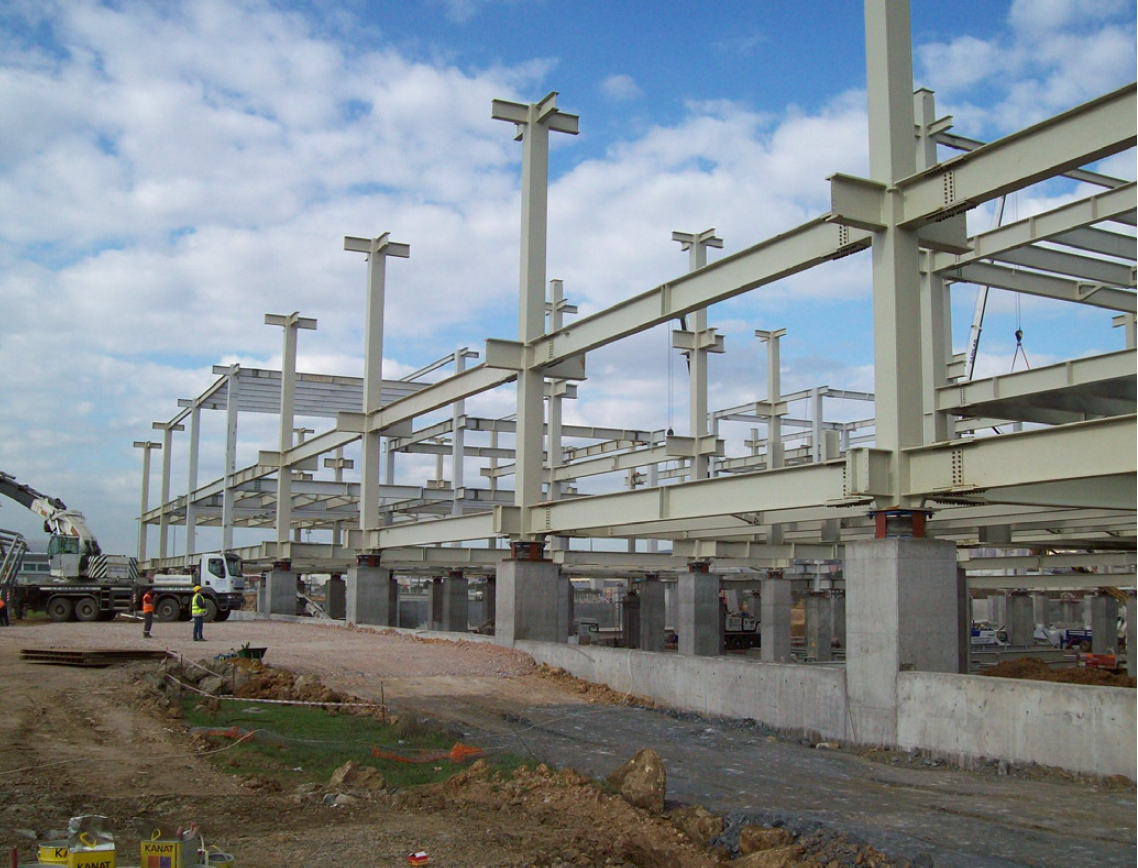
\includegraphics[scale=0.4]{b.PNG}
		\caption{A boat.}
		\label{fig:boat1}
\end{center}
\end{figure}


\blindtext

\blindtext

\blindtext

\blindtext

\blindtext \blindtext \blindtext \blindtext

\begin{table}[h!]
	\begin{center}
		\caption{Your first table.}
		\label{tab:table1}
		\begin{tabular}{l|c|r} % <-- Alignments: 1st column left, 2nd middle and 3rd right, with vertical lines in between
			\textbf{Value 1} & \textbf{Value 2} & \textbf{Value 3}\\
			$\alpha$ & $\beta$ & $\gamma$ \\
			\hline
			1 & 1110.1 & a\\
			2 & 10.1 & b\\
			3 & 23.113231 & c\\
		\end{tabular}
	\end{center}
\end{table}

\blindtext

\blindtext

\blindtext

\blindtext

\blindtext

\blindtext



\end{document}